\begin{figure}[H]
	\centering
	
\includegraphics[width=\linewidth]{samples/image.png}
\end{figure}

\begin{quote}
	\textbf{\LARGE ``}Lorem ipsum dolor sit amet, consectetur adipiscing elit. Praesent porttitor arcu luctus, imperdiet urna iaculis, mattis eros. Pellentesque iaculis odio vel nisl ullamcorper, nec faucibus ipsum molestie. Sed dictum nisl non aliquet porttitor. Etiam vulputate arcu dignissim, finibus sem et, viverra nisl. Aenean luctus congue massa, ut laoreet metus ornare in.\textbf{''}
	
	\hfill--- John Smith, 1972
\end{quote}



\begin{figure}[H]
	\centering
	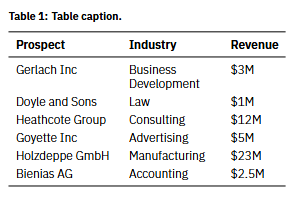
\includegraphics[width=\linewidth]{samples/image2.png}
\end{figure}


\begin{table}[H] % [H] forces the table to be output where it is defined in the code (it suppresses floating)
	\caption{Table caption.}
	\begin{tabular}{L{0.35\linewidth} L{0.31\linewidth} L{0.17\linewidth}} % Table column widths and alignment (L, C or R)
		\toprule
		\textbf{Prospect} & \textbf{Industry} & \textbf{Revenue} \\
		\midrule
		Gerlach Inc & Business Development & \$3M\\
		Doyle and Sons & Law & \$1M\\
		Heathcote Group & Consulting & \$12M\\
		Goyette Inc & Advertising & \$5M\\
		Holzdeppe GmbH & Manufacturing & \$23M\\
		Bienias AG & Accounting & \$2.5M\\
		\bottomrule
	\end{tabular}
	\label{tab:example}
\end{table}


\begin{figure}[H]
	\centering
	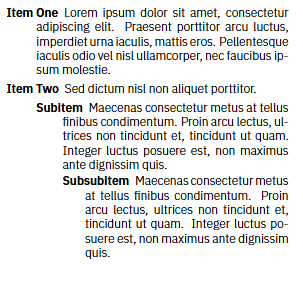
\includegraphics[width=\linewidth]{samples/image3.png}
\end{figure}


\begin{description}
	\item[Item One] Lorem ipsum dolor sit amet, consectetur adipiscing elit. Praesent porttitor arcu luctus, imperdiet urna iaculis, mattis eros. Pellentesque iaculis odio vel nisl ullamcorper, nec faucibus ipsum molestie. 
	\item[Item Two] Sed dictum nisl non aliquet porttitor.
	\begin{description}
		\item[Subitem] Maecenas consectetur metus at tellus finibus condimentum. Proin arcu lectus, ultrices non tincidunt et, tincidunt ut quam. Integer luctus posuere est, non maximus ante dignissim quis.
		\begin{description}
			\item[Subsubitem] Maecenas consectetur metus at tellus finibus condimentum. Proin arcu lectus, ultrices non tincidunt et, tincidunt ut quam. Integer luctus posuere est, non maximus ante dignissim quis.
	\end{description}
	\end{description}
	\item[Item Three] Etiam vulputate arcu dignissim, finibus sem et, viverra nisl. Aenean luctus congue massa, ut laoreet metus ornare in. Nunc fermentum nisi imperdiet lectus tincidunt vestibulum at ac elit. Nulla mattis nisl eu malesuada suscipit.
\end{description}


\begin{figure}[H]
	\centering
	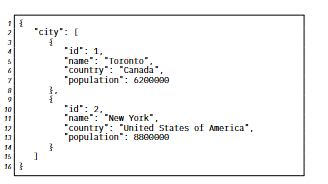
\includegraphics[width=\linewidth]{samples/image4.png}
\end{figure}

\begin{lstlisting}
{
	"city": [
		{
			"id": 1,
			"name": "Toronto",
			"country": "Canada",
			"population": 6200000
		},
		{
			"id": 2,
			"name": "New York",
			"country": "United States of America",
			"population": 8800000
		}
	]
}
\end{lstlisting}